Sprache lässt sich durch Grammatiken beschreiben und analysieren. Einfache Grammatik für einen kleinen Teil der deutschen Sprache:
\begin{itemize}
\item Satz $\to$ Nominalphrase Verbalphrase
\item Nominalphrase $\to$ Artikel Nomen
\item Artikel $\to$ die | eine
\item Nomen $\to$ katze | maus
\item Verbalphrase $\to$ Verb Nominalphrase
\item Verb $\to$ jagt | sieht
\end{itemize}
Damit lässt sich ableiten:
\begin{center}
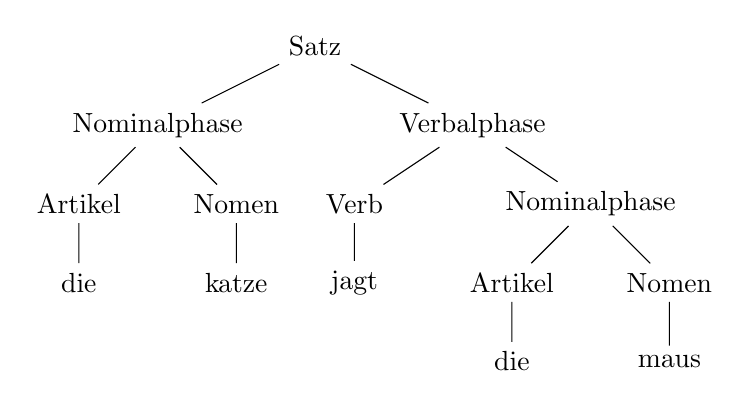
\begin{tikzpicture}[align=center]
\node (v1) at (0,0) {Satz};
\node (v2) at (-2,-1) {Nominalphase};
\node (v7) at (2,-1) {Verbalphase};
\node (v3) at (-3,-2) {Artikel};
\node (v4) at (-3,-3) {die};
\node (v5) at (-1,-2) {Nomen};
\node (v6) at (-1,-3) {katze};
\node (v8) at (0.5,-2) {Verb};
\node (v10) at (3.5,-2) {Nominalphase};
\node (v9) at (0.5,-3) {jagt};
\node (v11) at (2.5,-3) {Artikel};
\node (v13) at (4.5,-3) {Nomen};
\node (v12) at (2.5,-4) {die};
\node (v14) at (4.5,-4) {maus};
\draw (v1) -- (v2) -- (v3) -- (v4);
\draw (v2) -- (v5) -- (v6);
\draw (v1) -- (v7) -- (v8) -- (v9);
\draw (v7) -- (v10) -- (v11) -- (v12);
\draw (v10) -- (v13) -- (v14);
\end{tikzpicture}
\end{center}
Zur Darstellung von Strings verwenden wir Listen, zum Beispiel \lstinline$[die, katze, schläft]$.\\
Achtung: Wörter müssen klein geschrieben oder in \lstinline$"..."$ eingeschlossen werden, zum Beispiel \lstinline[language=Prolog]|["die", "Katze"]|.\\
Zur Darstellung der Grammatik verwenden wir einen Recursive Descent Parser (siehe Vorlesung TI). Idee dazu:\\
Die Grammatik-Prädikate haben die Form \lstinline$p(In, Rest)$. Dabei ist \lstinline$In$ die Eingabe. Das Prädikat \lstinline$p$ versucht einen Präfix der Eingabe entsprechend der Grammatikregeln, die \lstinline$p$ implementiert, zu verarbeiten. Der Rest der Eingabe, den \lstinline$p$ nicht verarbeitet hat, wird an \lstinline$Rest$ gebunden und ggf. als Eingabe an ein weiteres Grammatikprädikat weitergeleitet.
\cparagraph{Beispiel} $ $
\begin{lstlisting}[language=Prolog]
% Recursive Descent Parser für L = {a^n b^n | n >= 0  }
% Anfrage: s([a,a,a,b,b,b], []).

s(In, Rest) :-	% S -> aSb
	match(a, In, R1), 
	s(R1, R2),
	match(b, R2, Rest).
s(L, L).	% S -> epsilon

match(X, [X|Rest], Rest).
\end{lstlisting}
Beispiele:
\begin{lstlisting}[language=Prolog]
?- s([a,a,a,b,b,b], []).
true.
?- s([a,a,a,b,b,b], R). 
R = [b].
\end{lstlisting}

\cparagraph{Beispiel} $ $
\begin{lstlisting}[language=Prolog]
satz(In, Rest) :- nominal_phrase(In, R), verbal_phrase(R, Rest).
nominal_phrase(In, Rest) :- artikel(In, R), nomen(R, Rest).
verbal_phrase(In, Rest) :- verb(In, R), nominal_phrase(R, Rest).
artikel(In, Rest) :- match(eine, In, Rest); match(die, In, Rest).
verb(In, Rest) :- match(jagt, In, Rest); match(sieht, In, Rest).
nomen(In, Rest) :- match(katze, In, Rest); match(kater, In, Rest); match(maus, In, Rest).

match(X, [X|Rest], Rest).
\end{lstlisting}

\section{Genus-Kasus-Kongruenz}
In der vorherigen Katze-Maus Grammatik können grammatikalisch falsche Sätze erzeugt werden, zum Beispiel \lstinline`[die, kater, jagt, die maus]`.\\
Lösung: In der Nominalphrase müssen Artikel und Nomen in Genus und Kasus übereinstimmen. Wir führen Parameter \lstinline`Genus` und \lstinline`Kasus` in \lstinline`nominal_phrase` ein, die an \lstinline`artikel` und \lstinline`nomen` weitergeleitet werden. 

\subsection{Wertigkeit von Verben}
\lecdate{15.05.2017}
Zwei wichtige Klassen von Verben sind
\begin{itemize}
\item intransitives Verben: Diese führen kein Objekt nach sich (z.B. laufen, schlafen)
\item transitive Verben: Diese benötigen ein Objekt (z.B. (etwas) sehen, (etwas) fangen).
\end{itemize}
Das Verb bestimmt den Kasus des zugehörigen Objektes, z.B. jagen, fangen, sehen benötigen ein Akkusativobjekt (das Subjekt sieht wen oder was?).

\cparagraph{Beispiel} $ $
\begin{lstlisting}[language=Prolog]
satz(In, Rest) :- 
	nominal_phrase(_, nom, In, R), % Subjekt (Nominativ, wer oder was?) 
	verbal_phrase(R, Rest).

nominal_phrase(Genus, Kasus, In, Rest) :- 
	artikel(Genus, Kasus, In, R), nomen(Genus, R, Rest).

verbal_phrase(In, Rest) :- 
	verb_intransitiv(In, Rest);
	verb_transitiv(In, R), nominal_phrase(_, akk, R, Rest). % Objekt (Akkusativ, wen oder was?)

artikel(m, nom, In, Rest) :- match(A, In, Rest), member(A, [ein, der]).
artikel(f, nom, In, Rest) :- match(A, In, Rest), member(A, [eine, die]).
artikel(m, akk, In, Rest) :- match(A, In, Rest), member(A, [einen, den]).
artikel(f, akk, In, Rest) :- match(A, In, Rest), member(A, [eine, die]).

verb_intransitiv(In, Rest) :- match(V, In, Rest), member(V, [jagt, schläft, rennt]).
verb_transitiv(In, Rest) :- match(V, In, Rest), member(V, [jagt, sieht]).

nomen(m, In, Rest) :- match(kater, In, Rest).
nomen(f, In, Rest) :- match(V, In, Rest), member(V, [katze, maus]).

match(X, [X|Rest], Rest).
\end{lstlisting}





